\documentclass[12pt,a4paper]{article}

%--------------------------------------------------
% Packages de base
%--------------------------------------------------
\usepackage[utf8]{inputenc}
\usepackage[T1]{fontenc}
\usepackage[french]{babel}
\usepackage{amsmath, amssymb, amsfonts}
\usepackage{graphicx}
\usepackage{caption}
\usepackage{enumitem}
\usepackage{geometry}
\geometry{margin=2.5cm}
\usepackage{appendix}
\usepackage{tikz}
\usetikzlibrary{arrows.meta, positioning}
\newcommand{\quotes}[1]{``#1''}

\usepackage{hyperref}
\hypersetup{
    colorlinks,
    citecolor=black,
    filecolor=black,
    linkcolor=black,
    urlcolor=black
}

\usepackage{titling}
\renewcommand\maketitlehooka{\null\mbox{}\vfill}
\renewcommand\maketitlehookd{\vfill\null}

\title{\Huge{\textbf{Modèle de Cox-Ross-Rubinstein}}\\ \medskip
      \Huge{\textit{Notes}}\vspace*{0.7cm}}
\author{\LARGE{Alexis VO}\vspace{1cm}\\ \medskip
      Université Paris-Saclay\\École polytechnique}
\date{\vspace{0.2cm}\today}

%--------------------------------------------------
% Début du document
%--------------------------------------------------
\begin{document}
\renewcommand\labelitemi{\textbullet}

\maketitle

\newpage

\section*{Introduction}
Ces notes de cours sont rédigées durant mon stage en finance quantitative au CMAP de l'École polytechnique. Le sujet principal est le modèle binomial de Cox-Ross-Rubinstein. Ce document présente des concepts clés que le lecteur pourra enrichir. Il est recommandé au lecteur novice d'également se référer au glossaire. J'y développe les fondements, en expliquant de manière progressive les notions rencontrées.  Ce document est destiné à toute personne désirant comprendre les fondements du modèle binomial CRR et ses sujets connexes. Ma formation académique, une double-licence en mathématiques et informatique à l'université Paris-Saclay, me permet d'aborder ces éléments sans prérequis en finance. Je modélise également quelques simulations. Certaines notions fondamentales en mathématiques seront indispensables à la bonne compréhension de ce document.\\Bonne lecture.

\newpage

\tableofcontents

\newpage

%--------------------------------------------------
\section{Contexte et motivation}
En finance, il y a une multitude d'instruments permettant aux investisseurs de gérer les risques et de tirer parti des opportunités de marché. Parmi ces instruments, certains se distinguent par leur capacité à s'adapter aux fluctuations des \textit{actifs sous-jacents}. Ils ne nécessitent pas la possession directe de ces actifs. Ces instruments sont les \textit{produits dérivés}. Ils jouent un rôle essentiel dans les stratégies de \textit{couverture} et de \textit{spéculation}.

\subsection{Qu'est-ce qu'un \textit{produit dérivé} ?}
Un produit dérivé est un instrument financier dont la valeur dépend d'un actif dit \textit{sous-jacent}, comme une action ou une matière première. Par exemple,

\begin{itemize}
  \item Option d'achat (call)
  \item Option de vente (put)
\end{itemize}

\subsection{Pourquoi modéliser les prix ?}
Les marchés financiers sont incertains. Modéliser les prix permet :
\begin{itemize}
  \item d'anticiper les valeurs futures,
  \item de déterminer un \textit{juste prix} pour les produits dérivés,
  \item d'éviter les \textit{opportunités d'arbitrage}.
\end{itemize}
Nous y reviendrons tout au long de ce document.

\subsection{Présentation du modèle binomial}
Le modèle de Cox-Ross-Rubinstein (CRR), introduit en 1979 par ces auteurs, s'applique dans un cadre discret pour modéliser les mouvements d'un actif risqué. Ce modèle utilise une structure binomiale pour décrire l'évolution des prix d'un actif au fil du temps, ce qui signifie qu'à chaque étape, le prix de l'actif peut soit augmenter, soit diminuer selon un \textit{processus stochastique}.\\
\textbf{Remarque : } On retrouve bien cet aspect binomial, binaire : gain ou perte.

\begin{center}
    \begin{tikzpicture}[>=stealth, node distance=2.2cm and 3.2cm]

    \node (S0) at (0,0) {$S_0$};

    \node (Su1) at (3,2) {$S_0 \cdot u$};
    \node (Sd1) at (3,-2) {$S_0 \cdot d$};

    \node (Sun) at (7,3) {$S_0 \cdot u^n$};
    \node (Midn) at (7,0)   {$\cdots$};
    \node (Sdn) at (7,-3) {$S_0 \cdot d^n$};

    \draw[->] (S0) -- (Su1);
    \draw[->] (S0) -- (Sd1);

    \draw[dashed, ->] (Su1) -- (Sun);
    \draw[dashed, ->] (Su1) -- (Midn);
    \draw[dashed, ->] (Sd1) -- (Midn);
    \draw[dashed, ->] (Sd1) -- (Sdn);

    \node at (0,-3.5) {Temps $t = 0$};
    \node at (3,-3.5) {Temps $t = 1$};
    \node at (7,-3.5) {Temps $t = n$};

    \end{tikzpicture}
\end{center}

En décomposant ainsi le mouvement des prix en une série d'étapes discrètes, le modèle CRR permet de formaliser l'incertitude des marchés financiers de manière simplifiée. Au premier chef, cette première approche binomiale permet une meilleure compréhension du calcul des prix d'options et d'autres produits dérivés. Nous verrons dans un second temps comment ce modèle peut être généralisé.

%--------------------------------------------------
\section{Le modèle CRR à une période}

Le modèle CRR à une période -- ou bien \quotes{un pas deux états} -- introduit de manière simplifiée les concepts de modélisation financière en \textbf{temps discret}. Dans ce cadre, le modèle suppose qu'un actif financier peut évoluer selon deux états possibles sur une seule période : une \textit{hausse} ou une \textit{baisse} de prix. Le modèle à un pas deux états illustre les principes fondamentaux de l'\textit{arbitrage} et de l'\textit{évaluation neutre au risque}.

Nous verrons dans cette partie un exemple simple pour apprivoiser le modèle à un pas, puis nous le généraliserons dans la section suivante à un modèle à plusieurs périodes.

\subsection{Un exemple simple pour appréhender le modèle}

Considérons un actif dont le \textit{spot} est \( S_0 = 100\) euros. Supposons que dans un an, le prix de cet actif puisse soit augmenter de 20\% avec \( u = 1.2 \), soit diminuer de 10\% avec \( d = 0.9 \). Le taux d'intérêt sans risque est \( r = 0.05 \).

\begin{itemize}
    \item Prix initial (spot): \( S_0 = 100\) euros.
    \item Prix en cas de hausse : \( S_0 \cdot u = 120\) euros.
    \item Prix en cas de baisse : \( S_0 \cdot d = 90\) euros.
\end{itemize}

Supposons que nous ayons une option d'achat européenne -- un call européen -- avec un \textit{strike} de $105 euros$. Les valeurs de l'option à la fin de l'année sont :

\begin{itemize}
    \item \( V_u = \max(120 - 105, 0) = 15\) euros, si le prix monte.
    \item \( V_d = \max(90 - 105, 0) = 0\) euros, si le prix baisse.
\end{itemize}

\begin{center}
    \begin{tikzpicture}[>=stealth, node distance=2.5cm and 3.5cm]
    % Noeuds de prix de l'actif
    \node (S0)         at (0,0)       {$S_0 = 100$};
    \node (Su)         at (3,2)       {$S_u = 120$};
    \node (Sd)         at (3,-2)      {$S_d = 90$};

    % Noeuds de valeur de l'option
    \node (Vu)         at (6,2)       {$V_u = 15$};
    \node (Vd)         at (6,-2)      {$V_d = 0$};

    % Arêtes
    \draw[->] (S0) -- (Su) node[midway, above left] {u};
    \draw[->] (S0) -- (Sd) node[midway, below left] {d};
    \draw[->] (Su) -- (Vu);
    \draw[->] (Sd) -- (Vd);

    % Niveaux de temps
    \node at (0,-3) {$t=0$};
    \node at (3,-3) {$t=1$};
    \node at (6,-3) {maturity};

    \end{tikzpicture}
\end{center}

Jusque là, rien de bien compliqué. Nous avons un actif dont le prix peut évoluer de deux manières possibles, et nous avons calculé la valeur d'une option d'achat européenne à l'échéance. Voyons désormais comment évaluer cette option en utilisant la probabilité neutre au risque.

\subsection{Théorème fondamental de l'évaluation des actifs}

Dans le cadre général du modèle binomial à un pas, nous cherchons à évaluer un produit dérivé en utilisant une probabilité neutre au risque. On supposera l'absence d'opportunité d'arbitrage. Cette hypothèse est forte.

\begin{itemize}
    \item \( S_0 \) : Prix initial de l'actif.
    \item \( u \) et \( d \) : Facteurs de hausse et de baisse.
    \item \( r \) : Taux d'intérêt sans risque.
\end{itemize}

Le théorème d'évaluation neutre au risque donne que la valeur initiale \( V_0 \) du produit dérivé est :

\begin{equation}
    \boxed{V_0 = \frac{1}{1 + r} \left( q \cdot V_u + (1 - q) \cdot V_d \right)}
\end{equation}

où \( q \) est la probabilité neutre au risque définie par :

\begin{equation}
    \boxed{q = \frac{(1 + r) - d}{u - d}}
\end{equation}

\vspace{1cm}

\begin{center}
    \begin{tikzpicture}[>=stealth, node distance=2cm and 3.5cm, thick]
        \node (V0) at (0,0) {$V_0$};
        \node (Vu) at (4,2) {$V_u$};
        \node (Vd) at (4,-2) {$V_d$};

        \draw[->, dashed] (Vu) -- (V0) node[midway, above left] {$q$};
        \draw[->, dashed] (Vd) -- (V0) node[midway, below left] {$1 - q$};

        \node at (0,-3) {$t=0$};
        \node at (4,-3) {$t=1$};
    \end{tikzpicture}\\
    \textbf{Évaluation au temps $t = 0$ à partir de $t = 1$}
\end{center}

Ce théorème repose sur l'idée que, sous la probabilité neutre au risque, le rendement attendu de l'actif risqué est égal au taux d'intérêt sans risque. Cela permet d'évaluer le produit dérivé en actualisant les paiements futurs à leur valeur présente.

\subsection{Démonstration}

Pour démontrer ce théorème, nous allons construire un \textit{portefeuille répliquant} qui reproduit les gains du produit dérivé. Ce portefeuille constitue une \textbf{stratégie de couverture parfaite}, car il permet d’éliminer totalement le risque de marché associé au produit dérivé.
Il est composé de deux éléments : une position dans \textbf{l'actif risqué} et une position dans un \textbf{actif sans risque}.

\subsubsection{Construction d'une stratégie de couverture par réplication}

Considérons un portefeuille composé de \(\Delta\) unités de l'actif risqué (action) et d'un montant \(B\) investi dans un actif sans risque (obligation). On suppose que ce portefeuille est \textbf{auto-financé}, c’est-à-dire que ses variations de valeur proviennent uniquement de la revalorisation des actifs détenus, sans nouvel apport externe.\\

La valeur initiale du portefeuille est :
\begin{equation}
\boxed{V_0 = \Delta \cdot S_0 + B}
\end{equation}

À la fin de la période, la valeur du portefeuille évolue en fonction de la variation du prix de l'actif risqué :

\begin{itemize}
    \item Si le prix de l'actif monte, la valeur du portefeuille devient \(\Delta \cdot S_0 \cdot u + B \cdot (1 + r)\).
    \item Si le prix de l'actif baisse, la valeur du portefeuille devient \(\Delta \cdot S_0 \cdot d + B \cdot (1 + r)\).
\end{itemize}

\noindent \textbf{Objectif de la couverture :} Construire \((\Delta, B)\) tels que, quelle que soit l’évolution du sous-jacent, la valeur du portefeuille soit exactement égale à celle de l’option à l’échéance. Cela revient à éliminer tout risque de marché : le portefeuille « couvre » les fluctuations du sous-jacent.

\subsubsection{Réplication du produit dérivé}

Soit \(V_u\) la valeur du produit dérivé si le sous-jacent monte, et \(V_d\) s’il baisse. On impose :
\begin{align}
\Delta \cdot S_0 \cdot u + B \cdot (1 + r) &= V_u \\
\Delta \cdot S_0 \cdot d + B \cdot (1 + r) &= V_d
\end{align}

On soustrait les deux équations pour éliminer \(B\) :
\[
\Delta \cdot S_0 \cdot (u - d) = V_u - V_d
\]
d'où :
\begin{equation}
\boxed{\Delta = \frac{V_u - V_d}{S_0 \cdot (u - d)}}
\end{equation}

Puis on substitue \(\Delta\) pour trouver \(B\) :
\begin{equation}
\boxed{B = \frac{u \cdot V_d - d \cdot V_u}{(1 + r) \cdot (u - d)}}
\end{equation}

\noindent \textbf{Interprétation de \(\Delta\) :} Il représente la quantité d’actif risqué nécessaire pour couvrir une variation du prix du produit dérivé -- d’où son nom : \textbf{Delta}, dérivée du prix de l’option par rapport au sous-jacent.

\subsubsection{Valeur initiale et stratégie de couverture}

On rappelle la valeur initiale du portefeuille répliquant (et donc de l’option) :
\[
V_0 = \Delta \cdot S_0 + B
\]

En remplaçant \(\Delta\) et \(B\), on obtient :
\[
V_0 = \frac{(1 + r - d) \cdot V_u + (u - (1 + r)) \cdot V_d}{(1 + r) \cdot (u - d)}
\]

Ce résultat met en évidence que le prix d’un dérivé correspond à l’espérance sous une probabilité fictive, la \textit{probabilité neutre au risque} \(q\), définie comme :
\begin{equation}
\boxed{q = \frac{(1 + r) - d}{u - d}, \qquad 1 - q = \frac{u - (1 + r)}{u - d}}
\end{equation}

\subsubsection{Évaluation neutre au risque}

On réécrit alors le prix initial sous forme probabiliste :
\begin{equation}
\boxed{V_0 = \frac{1}{1 + r} \left( q \cdot V_u + (1 - q) \cdot V_d \right)}
\label{eq:prix_option}
\end{equation}

Ce résultat montre que la stratégie de couverture \((\Delta, B)\) permet de \textit{reproduire exactement} le payoff du dérivé, et donc que sa valeur actuelle est l’espérance actualisée de sa valeur future, sans arbitrage.

\begin{flushright}
\begin{tikzpicture}
\draw[fill=white] (0,0) rectangle (0.25cm,0.25cm);
\end{tikzpicture}
\end{flushright}

%--------------------------------------------------

\subsection{Interprétation}

Analysons la formule \eqref{eq:prix_option} :

\begin{itemize}
    \item \textbf{Actualisation} : Le facteur \(\frac{1}{1 + r}\) actualise les paiements futurs à leur valeur présente. Par exemple, un euro reçu dans le futur pourrait valoir moins qu'un euro reçu aujourd'hui.
    \item \textbf{Probabilité neutre au risque} : La probabilité \( q \) est calculée de manière à ce que l'espérance du rendement de l'actif sous-jacent soit égale au taux sans risque. Cela élimine le risque de marché et permet une évaluation cohérente des produits dérivés.
    \item \textbf{Espérance des paiements} : Le terme \( q \cdot \text{V}_u + (1 - q) \cdot \text{V}_d \) représente l'espérance des paiements futurs du produit dérivé sous la probabilité neutre au risque.

\end{itemize}
\textbf{Remarque :} le prix actualisé est une \textbf{martingale} sous la probabilité neutre au risque. En effet, le prix du produit dérivé ne présente pas de tendance haussière ni baissière dans le temps, ce qui est une condition essentielle pour éviter les opportunités d'arbitrage.

\vspace{0.25cm}

Nous étendrons par la suite ce \textit{modèle à un pas deux états} à un modèle multi-périodes et à d'autres types de modèles financiers. Mais avant, appliquons ce que nous venons de voir à l'exemple d'introduction.

\subsection{Exemple récapitulatif}

On rappelle que nous avons un call européen avec les données suivantes :

\subsubsection{Données initiales}
\begin{itemize}
    \item Spot : \( S_0 = 100\) euros.
    \item Strike : \( K = 105\) euros.
    \item Facteur de hausse : \( u = 1,2 \).
    \item Facteur de baisse : \( d = 0,9 \).
    \item Taux d'intérêt sans risque : \( r = 0,05 \).
\end{itemize}
On avait établit que le payoff du call à l'échéance est :
\begin{itemize}
    \item Payoff en cas de hausse : \( V_u = \max(S_u - K, 0) = \max(120 - 105, 0) = \textbf{15}\) euros.
    \item Payoff en cas de baisse : \( V_d = \max(S_d - K, 0) = \max(90 - 105, 0) = \textbf{0}\) euros.
\end{itemize}

\subsubsection{Évaluation neutre au risque}
On calcule la probabilité neutre au risque \( q \) :
\[ q = \frac{(1 + r) - d}{u - d} = \frac{(1 + 0,05) - 0,9}{1,2 - 0,9} = \frac{0,5}{0,3} = \textbf{0,5} \]

\subsubsection{Calcul du prix de l'option}
Le prix du call est calculé en utilisant la formule d'évaluation neutre au risque démontrée précédemment:
\[ V_0 = \frac{1}{1,05} \left( 0,5 \cdot 15 + (1 - 0,5) \cdot 0 \right) \]
\[ V_0 = \frac{1}{1,05} \left( 7,5 \right) \]
\[ \boxed{V_0 \approx 7,14 \text{ euros}} \]

\subsubsection{Conclusion et interprétations}

Dans cet exemple, le prix du call européen est d’environ \( 7{,}14 \) euros. Voici quelques stratégies et interprétations qui permettent de mieux saisir le rôle et l’intérêt d’une option d’achat.

\begin{itemize}

    \item \textbf{Stratégie de spéculation}

    \begin{itemize}
        \item \textbf{Parier sur une hausse} : acheter ce call revient à parier que le prix de l’actif dépassera 105 euros. Si par exemple, l’actif monte à 120 euros, le call vaudra 15 euros à l’échéance. On gagne donc \( 15 - 7{,}14 = 7{,}86 \) euros.
        
        \item \textbf{Effet de levier} : l’option permet d’investir peu (7,14 €) pour viser un gain plus grand. C'est un \textbf{effet de levier} : un petit investissement peut rapporter beaucoup, ou être perdu entièrement.
    \end{itemize}

    \item \textbf{Stratégie de couverture}

    \begin{itemize}
        \item \textbf{Se protéger contre une hausse} : si on est vendeur de l’actif -- position courte i.e. on vend un actif que l’on ne possède pas, dans l’espoir de le racheter plus tard à un prix plus bas pour faire un profit -- une option call peut servir de protection. En cas de hausse, les pertes sur la position courte sont compensées par les gains sur l’option.
        
        \item \textbf{Vue comme une assurance} : acheter un call peut s’interpréter comme une assurance contre une hausse du prix. La prime (7,14 €) est le “coût” de cette assurance.
    \end{itemize}

    \item \textbf{Pas d’arbitrage possible}. Le prix de l’option est calculé en supposant qu’il n’existe pas de stratégie d’arbitrage, c’est-à-dire pas de moyen de gagner de l’argent sans risque. Ce principe est fondamental.

    \item \textbf{Lien entre risque et rendement}

    \begin{itemize}
        \item Le prix de l’option reflète le risque pris par l’acheteur : si le scénario favorable ne se réalise pas, il perd sa mise.
        
        \item En contrepartie, il existe un rendement potentiel important si le prix monte beaucoup. L’investisseur doit donc estimer si "le jeu en vaut la chandelle".
    \end{itemize}
\end{itemize}

\textbf{Conclusion}. Cet exemple nous a permis de comprendre pourquoi les options sont utilisées : soit pour prendre une position réfléchie, soit pour se couvrir contre un risque, avec un contrôle clair des pertes possibles. \textbf{Mot-clé :} assurance.

%--------------------------------------------------
%--------------------------------------------------
\section{Le modèle CRR à plusieurs périodes}

On s'intéresse désormais au modèle CRR à plusieurs périodes.

\subsection{Structure de l'arbre binomial}
Dans un modèle CRR à $n$ périodes, à chaque date $t \in \{0,1,2,\dots,n\}$, le prix de l'actif peut évoluer en suivant une structure d'arbre binomial :

\begin{itemize}
    \item À chaque étape, le prix monte d'un facteur $u > 1$ ou baisse d'un facteur $d < 1$.
    \item Ainsi, au temps $t$, un chemin donné correspond à $i$ hausses et $(t-i)$ baisses.
    \item Le prix de l'actif après $i$ hausses est :
    \(
    \boxed{S_t^{(i)} = S_0 \cdot u^i \cdot d^{t-i}}
    \)
    \item On conserve l'hypothèse d'absence d'arbitrage. On définit la probabilité neutre au risque $q$ comme précédemment :
    \(
    q = \frac{(1 + r) - d}{u - d}.
    \)
    Cette probabilité reste constante à chaque étape.
\end{itemize}


\subsection{Évaluation d'une option européenne}
Soit $V_t^{(i)}$ la valeur de l'option à la date $t$ au noeud correspondant à $i$ hausses.
L'évaluation se fait par \textbf{backward induction}, en remontant de la maturité $t = n$ jusqu'à $t = 0$ :

\begin{itemize}
  \item On connaît la valeur de l'option à maturité $T = n$.
  \item On applique la formule de récurrence connue suivante
  \[
    V_t^{(i)} = \frac{1}{1 + r} \left( q \cdot V_{t+1}^{(i+1)} + (1 - q) \cdot V_{t+1}^{(i)} \right)
  \]
  \item \textbf{Valeur initiale} : $V_0 = V_0^{(0)}$
\end{itemize}

\subsection{Pseudo-code d'implémentation}
Pour implémenter l'évaluation d'une option européenne dans le modèle CRR à $n$ périodes, on peut utiliser un tableau pour stocker les valeurs de l'actif et de l'option à chaque étape. Voici une proposition de pseudo-code.
\begingroup\small
\begin{verbatim}
@Input :
n : nombre de périodes
u, d : facteurs de montée et descente du prix de l’actif
r : taux d’intérêt sans risque par période
S0 : prix initial de l’actif
K : prix d’exercice de l’option
payoff(S) : fonction payoff de l’option
(ex: max(S-K, 0) pour un call européen)

# Initialisation :
q = ((1 + r) - d) / (u - d)  # probabilité neutre au risque

# Étape 1 : calcul des valeurs possibles de l’actif à maturité
pour i de 0 à n :
    S[n][i] = S0 * u^i * d^(n - i)
    V[n][i] = payoff(S[n][i])  # valeur de l’option à maturité

# Étape 2 : remontée de l’arbre (backward induction)
pour t de n-1 à 0 par pas -1 :
    pour i de 0 à t :
        V[t][i] = (1 / (1 + r)) * ( q * V[t+1][i+1] + (1 - q) * V[t+1][i] )

@Output :
V[0][0]  # valeur de l’option à la date initiale
\end{verbatim}
\endgroup

\subsection{Exemple d'arbre pour n=2}
\begin{center}
\begin{tikzpicture}[>=stealth, node distance=2.2cm and 2.5cm]
  % Niveau t=0
  \node (S00) at (0,0) {$S_0$};

  % Niveau t=1
  \node (S10) at (2,1.5) {$S_0 u$};
  \node (S11) at (2,-1.5) {$S_0 d$};

  % Niveau t=2
  \node (S20) at (4,3) {$S_0 u^2$};
  \node (S21) at (4,0) {$S_0 ud$};
  \node (S22) at (4,-3) {$S_0 d^2$};

  \draw[->] (S00) -- (S10);
  \draw[->] (S00) -- (S11);
  \draw[->] (S10) -- (S20);
  \draw[->] (S10) -- (S21);
  \draw[->] (S11) -- (S21);
  \draw[->] (S11) -- (S22);

  \node at (0,-4) {$t=0$};
  \node at (2,-4) {$t=1$};
  \node at (4,-4) {$t=2$};
\end{tikzpicture}
\end{center}

\subsection{Complexité}
Le modèle binomial est intuitif et simple à mettre en œuvre. Cependant, il présente certaines limites importantes. Le nombre de nœuds dans l’arbre croît rapidement avec le nombre de périodes : sans recombinaison, il atteint \(2^{n+1} - 1\) pour \(n\) périodes, ce qui induit une complexité exponentielle en mémoire. Même dans sa version recombinante, le modèle conserve une complexité temporelle et spatiale de l’ordre de \(O(n^2)\), ce qui peut rendre les calculs coûteux pour des valeurs élevées de \(n\).

\begin{center}
    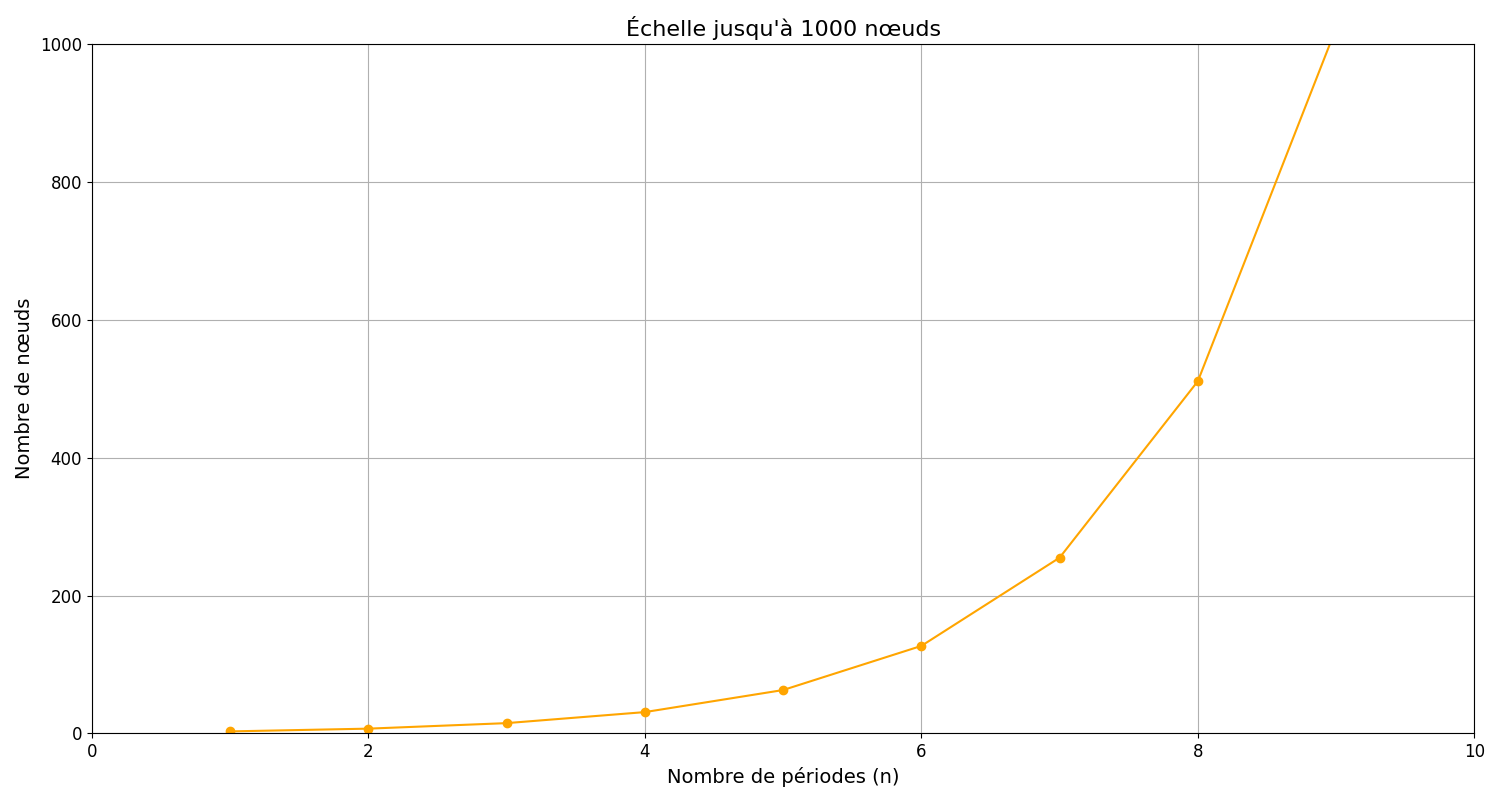
\includegraphics[width=1\textwidth]{lim.png}
\end{center}

Par ailleurs, la précision de l’évaluation dépend fortement du choix des paramètres \(u\), \(d\) et \(r\), ainsi que de la fonction de payoff considérée. Le modèle repose sur des hypothèses simplificatrices, notamment une \textit{volatilité constante}, et ne prend pas en compte des phénomènes plus réalistes comme la \textit{volatilité stochastique} ou d’autres facteurs de marché. Ces limitations réduisent donc la pertinence du modèle binomial pour des produits financiers complexes ou dans des contextes de marché plus instables.

\subsection{Exemple d'application}
\noindent \textbf{Données}. On considère une option d’achat (call) européenne, tel que :

\begin{itemize}
    \item Prix initial de l’action : $S_0 = 100$
    \item Prix d’exercice : $K = 100$
    \item Durée : $T = 2$ périodes
    \item Facteur de hausse : $u = 1.2$
    \item Facteur de baisse : $d = 0.8$
    \item Taux sans risque par période : $r = 0.05$
\end{itemize}

Dans cet exemple, on cherche à déterminer la valeur de l'option (européenne) à \(t = 0\).

\noindent \textbf{Étape 1 : Probabilité neutre au risque}. La probabilité neutre au risque $q$ est donnée par :
\[
q = \frac{(1 + r) - d}{u - d} = \frac{1.05 - 0.8}{1.2 - 0.8} = \frac{0.25}{0.4} = \textbf{0.625}
\]

\noindent \textbf{Étape 2 : Arbre des prix de l’actif}. On construit l’arbre du prix de l’actif :

\[
\begin{array}{ccc}
\text{Temps 0} & \text{Temps 1} & \text{Temps 2} \\
S_0 = 100 & \begin{cases}
S_u = 120 \\
S_d = 80
\end{cases}
&
\begin{cases}
S_{uu} = 144 \\
S_{ud} = S_{du} = 96 \\
S_{dd} = 64
\end{cases}
\end{array}
\]

\noindent \textbf{Étape 3 : Valeur de l’option à maturité (temps 2)}. L’option d’achat donne un gain de $\max(S_T - K, 0)$. On obtient donc :

\[
\begin{aligned}
V_{uu} &= \max(144 - 100, 0) = 44 \\
V_{ud} = V_{du} &= \max(96 - 100, 0) = 0 \\
V_{dd} &= \max(64 - 100, 0) = 0
\end{aligned}
\]

\noindent \textbf{Étape 4 : Backward induction}. On remonte à l’instant $t=1$ en utilisant la formule :
\[
V = \frac{1}{1 + r} \left[ q \cdot V_\text{haut} + (1 - q) \cdot V_\text{bas} \right]
\]

\textit{Noeud haut à $t=1$ (prix = 120)} :
\[
V_u = \frac{1}{1.05} \left[ q \cdot 44 + (1 - q) \cdot 0 \right] = \frac{1}{1.05} (0.625 \cdot 44) = \frac{27.5}{1.05} \approx 26.19
\]

\textit{Noeud bas à $t=1$ (prix = 80)}
\[
V_d = \frac{1}{1.05} \left[ q \cdot 0 + (1 - q) \cdot 0 \right] = 0
\]

\textit{Noeud initial à $t=0$ (prix = 100)}
\[
V_0 = \frac{1}{1.05} \left[ q \cdot V_u + (1 - q) \cdot V_d \right] = \frac{1}{1.05} (0.625 \cdot 26.19) \approx \frac{16.37}{1.05} \approx 15.59
\]

\paragraph{Résultat final} La valeur de l’option d’achat européenne à $t=0$ est environ :
\[\boxed{15.59 \text{ euros}}\]

\paragraph{Interprétation des résultats.} Avec deux périodes, on obtient \( 2^2 + 1 = 5 \) nœuds, et la recombinaison (\( S_{ud} = S_{du} \)) réduit de façon négligeable la complexité. On voit qu’un seul scénario (la double hausse) mène à un payoff positif de l’option.

D'autre part, on observe une décroissance des valeurs d’option en remontant dans l’arbre : \( V_{uu} = 44 \), puis \( V_u \approx 26{,}19 \), puis \( V_0 \approx 15{,}59 \). Cela reflète le fait que plus on est loin de la maturité, plus l'incertitude est grande et plus la valeur actuelle est faible (effet d’actualisation).
    
Enfin, on constate que même pour un nombre réduit de périodes, il y a un certains nombre de calculs : c'est long. Cela met en évidence d'une part la nécessité d'une implémentation numérique, et d'autre part, un modèle plus adapté pour un nombre élevé de périodes.


%--------------------------------------------------

\section{Vers le modèle de Black-Scholes...}

L'approche avec le modèle binomial de CRR à plusieurs périodes présente plusieurs avantages. La première est qu'elle permet de mieux modéliser la dynamique des prix d'un actif sur une période plus longue, en tenant compte des fluctuations possibles à chaque étape. De plus, elle offre une flexibilité pour évaluer des options avec des caractéristiques plus complexes, comme les options américaines qui peuvent être exercées à tout moment avant l'échéance. Nous verrons cela dans une prochaine section. Enfin, cette approche permet de se rapprocher du \textbf{modèle de Black-Scholes} en faisant tendre le nombre de périodes $n$ vers l'infini, ce qui conduit à une approximation continue des mouvements de prix. Il sera évoqué dans un autre chapitre.
\begin{center}
    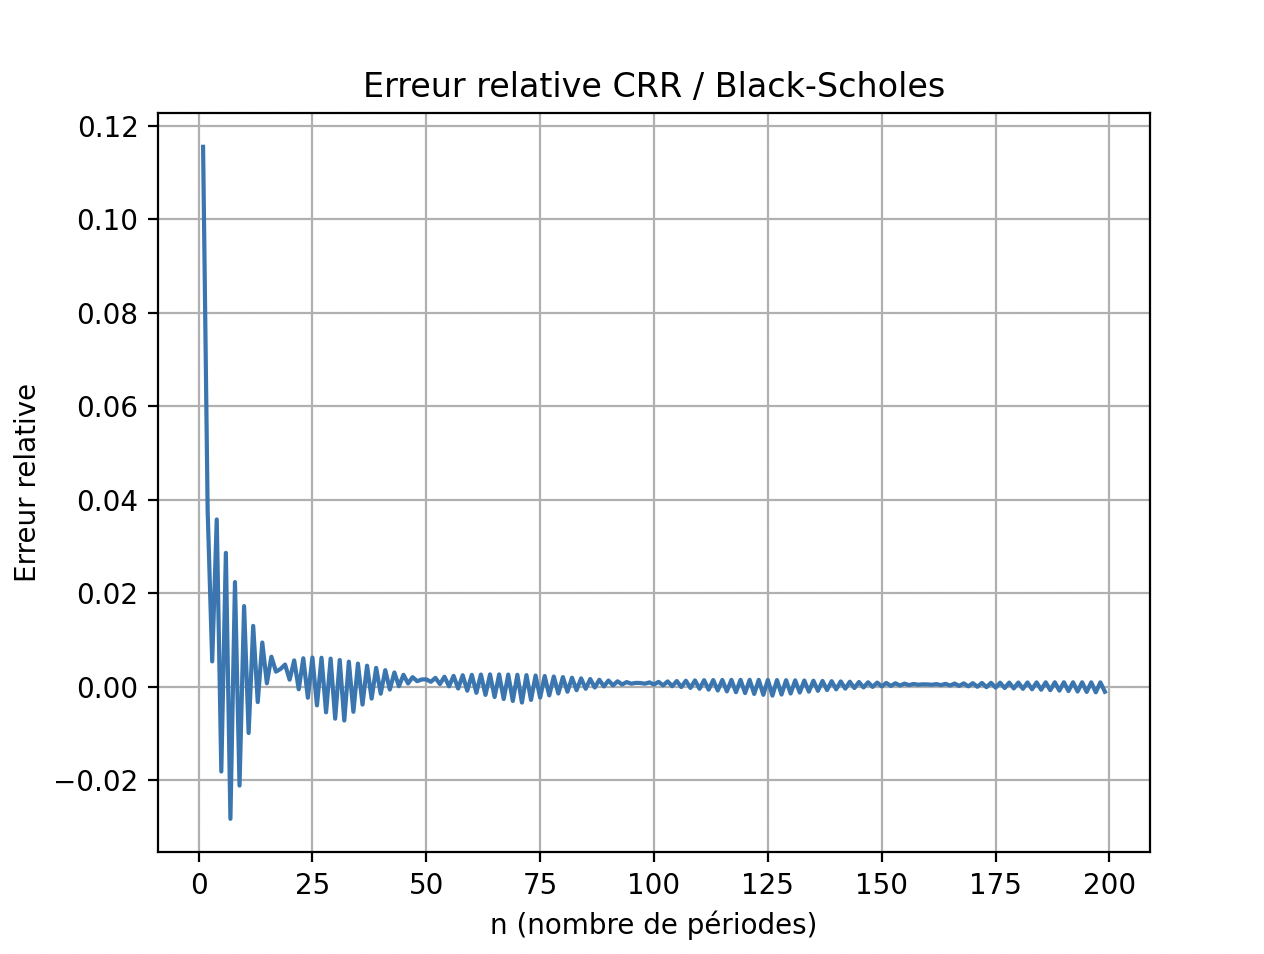
\includegraphics[width=0.8\textwidth]{../tp_crr/error_plot.png}
    \captionof*{figure}{D'après le TP MAP552 réalisé en Python.}
\end{center}

\paragraph{Lien avec le delta-hedging en temps continu.} Le modèle binomial de CRR fournit une version discrète de la stratégie de couverture continue utilisée avec le modèle de Black-Scholes. En effet, à chaque pas de temps, la position \(\Delta_t\) est ajustée dynamiquement en fonction de la configuration de l’arbre.

Quand le nombre de pas \(n \to \infty\), on peut montrer que :
\[
\boxed{\Delta_t^{\text{CRR}} \longrightarrow \frac{\partial V}{\partial S}(t, S_t)}
\]
où le membre de droite est le \textbf{delta de Black-Scholes}.\\

Ainsi, le modèle CRR constitue une \textbf{approximation naturelle du delta-hedging} en temps discret.



%--------------------------------------------------
\section{Extensions du modèle CRR à d'autres types d'options}

Le modèle binomial de Cox-Ross-Rubinstein s'applique également pour traiter d'autres instruments dérivés. Le principe général -- construire un arbre de recombinaison des prix, puis utiliser une induction en arrière (backward induction) sous la probabilité neutre au risque -- demeure identique. Néanmoins, certaines spécificités doivent être prises en compte selon le type d'option.

\subsection{Option de vente européenne (put)}
Le raisonnement est identique à celui du call, mais le payoff est différent. Pour une option de vente européenne (put), le gain à maturité est :
\[
\boxed{\max(K - S_T, 0)}
\]
On procède de la même manière :
\begin{enumerate}
    \item Construction de l’arbre des prix de l’actif.
    \item Calcul du payoff terminal avec la formule du put.
    \item Remontée dans l’arbre avec la formule d’induction.
\end{enumerate}

\subsection{Options américaines}
Les options américaines (call ou put) peuvent être exercées à tout moment \textbf{avant ou à l’échéance}. Cela modifie la backward induction : à chaque nœud, il faut comparer la \textbf{valeur de continuation} avec la \textbf{valeur intrinsèque}, et prendre le maximum des deux :
\[
\boxed{V = \max\left( \text{valeur intrinsèque}, \, \frac{1}{1 + r} \left[ q V_\text{haut} + (1 - q) V_\text{bas} \right] \right)}
\]
Cela rend le modèle un peu plus complexe, car il faut tester cette condition à chaque étape de l’induction.

\subsection{Cas généraux et autres payoffs}
Le modèle CRR peut être utilisé pour tout produit dérivé dont le payoff dépend du prix de l’actif sous-jacent à des dates discrètes. Voici quelques exemples :
\begin{itemize}
    \item \textbf{Options asiatiques (arithmétiques ou géométriques)} : le payoff dépend de la moyenne des prix passés. L’arbre devient plus complexe car il faut stocker l’historique ou des agrégats.
    \item \textbf{Options barrières} : l’option n’a de valeur que si une certaine barrière est franchie ou non. L’arbre est filtré en fonction de la barrière.
    \item \textbf{Options lookback} : dépendent du maximum ou minimum atteint par le sous-jacent. Là aussi, il faut enrichir l’état de chaque nœud.
\end{itemize}



%--------------------------------------------------

\newpage 

\section{Conclusion}

Le modèle binomial de Cox-Ross-Rubinstein (CRR) -- ou modèle binomial -- est une approche pour la valorisation des options en temps discret. Il modélise l’évolution du prix d’un actif par un arbre binaire. De plus, le modèle binomial permet d’estimer la valeur d’options européennes, américaines ou plus complexes grâce à l’induction en arrière (backward induction) sous la probabilité neutre au risque. Pour pouvoir appliquer cette méthode, il faut faire l'hypothèse forte de l'absence d'arbitrage et actualiser les flux financiers. Toutefois, l’approche CRR présente des limites : la taille de l’arbre croît de manière exponentielle avec le nombre de périodes, ce qui peut entraîner une complexité importante. D'autre part, le modèle repose sur des hypothèses simplificatrices telles que la volatilité constante ou encore le marché frictionless. Ceci le rend inadapté à certains contextes de marché réels.

Ce travail constitue une première étape vers des outils plus puissants de la finance quantitative. Le passage à la limite du modèle binomial, nous conduit à étudier le modèle de Black-Scholes en temps continu. Ce dernier introduit les équations différentielles stochastiques et la formule de Black-Scholes-Merton, pierre angulaire de la théorie moderne des options. D’autres prolongements incluent les modèles avec volatilité stochastique, les modèles à sauts, ou encore l’étude de la couverture dynamique (hedging), tous mobilisant des outils mathématiques avancés tels que l’Itô-calcul, la théorie de mesure équivalente, et les martingales.

\newpage

%--------------------------------------------------
\appendix
%--------------------------------------------------

\section{Préliminaires mathématiques}
\subsection*{1. Probabilités et variables aléatoires}

\begin{itemize}
    \item \textbf{Arbre binomial et processus stochastiques discrets} : compréhension de la structure d’un arbre de probabilités avec deux états (hausse/baisse) par période, et des chemins possibles.
    \item \textbf{Espérance conditionnelle} : savoir calculer l’espérance d’une variable aléatoire en fonction d’une information passée.
\end{itemize}

\subsection*{2. Analyse mathématique et calculs financiers}

\begin{itemize}
    \item \textbf{Actualisation et valeur temps de l'argent} : capacité à calculer la valeur actuelle d’un flux futur.
    \item \textbf{Induction arrière (backward induction)} : technique de calcul rétrograde, utilisée pour remonter l’arbre à partir de la valeur de l’option à maturité.
\end{itemize}

\subsection*{3. Notions spécifiques en finance mathématique}

\begin{itemize}
    \item \textbf{Portefeuille auto-financé et absence d’arbitrage} : savoir construire un portefeuille répliquant, et comprendre qu’un modèle sans arbitrage ne permet pas de profits sans risque.
    \item \textbf{Loi du prix unique} : principe selon lequel deux portefeuilles répliquant le même payoff doivent avoir la même valeur aujourd’hui.
\end{itemize}

\subsection*{4. Combinatoire et formules binomiales (facultatif)}

\begin{itemize}
    \item \textbf{Formule binomiale} : pour des arbres de grande taille, il est possible d’utiliser directement la formule :
    \[
    V_0 = \frac{1}{(1 + r)^n} \sum_{k=0}^{n} \binom{n}{k} q^k (1-q)^{n-k} \cdot \text{payoff au nœud}
    \]
\end{itemize}

\section{TP CRR - MAP552}
TODO : insérer le fichier du TP réalisé en Python.

%--------------------------------------------------
\section{Exercices}

\subsection*{Exercice 1 -- Call européen sur 1 période}
On considère une option d’achat européenne avec les données suivantes :

\begin{itemize}
    \item Prix initial de l’action : $S_0 = 100$
    \item Prix d’exercice : $K = 105$
    \item Durée : $T = 1$ période
    \item Facteur de hausse : $u = 1.1$
    \item Facteur de baisse : $d = 0.9$
    \item Taux sans risque : $r = 0.05$
\end{itemize}

\textbf{Question} : Calculer la valeur de l’option d’achat à $t = 0$.

\vspace{0.3cm}

\subsection*{Exercice 2 — Put européen sur 2 périodes}
On considère une option de vente européenne avec les paramètres suivants :

\begin{itemize}
    \item $S_0 = 50$, $K = 52$, $T = 2$ périodes
    \item $u = 1.2$, $d = 0.8$, $r = 0.05$
\end{itemize}

\textbf{Question} : Construire l’arbre des prix, puis celui des valeurs du put, et en déduire la valeur de l’option à $t = 0$.

\vspace{0.3cm}

\subsection*{Exercice 3 — Option américaine à 3 périodes}
On considère une option de vente \textbf{américaine} sur 3 périodes avec :

\begin{itemize}
    \item $S_0 = 40$, $K = 42$, $T = 3$ périodes
    \item $u = 1.2$, $d = 0.85$, $r = 0.04$
\end{itemize}

\textbf{Question} : Calculer la valeur de l’option en considérant la possibilité d’exercice anticipé à chaque étape. Identifier à quel(s) nœud(s) il est optimal d’exercer.

\vspace{1cm}

\subsection*{Correction des exercices}

\subsubsection*{Correction de l’exercice 1}

\textbf{Étape 1 : Calcul de la probabilité neutre au risque}

\[
q = \frac{(1 + r) - d}{u - d} = \frac{1.05 - 0.9}{1.1 - 0.9} = \frac{0.15}{0.2} = 0.75
\]

\textbf{Étape 2 : Valeurs à maturité}

\[
\begin{aligned}
S_u &= 100 \times 1.1 = 110 \Rightarrow V_u = \max(110 - 105, 0) = 5 \\
S_d &= 100 \times 0.9 = 90 \Rightarrow V_d = \max(90 - 105, 0) = 0
\end{aligned}
\]

\textbf{Étape 3 : Valeur actuelle}

\[
V_0 = \frac{1}{1.05} \left(0.75 \cdot 5 + 0.25 \cdot 0\right) = \frac{3.75}{1.05} \approx \boxed{3.57}
\]

\vspace{0.5cm}

\subsection*{Correction de l’exercice 2}

\textbf{Étape 1 : Probabilité neutre au risque}

\[
q = \frac{1.05 - 0.8}{1.2 - 0.8} = \frac{0.25}{0.4} = 0.625
\]

\textbf{Étape 2 : Arbre des prix}

\[
\begin{aligned}
S_{uu} &= 50 \cdot 1.2^2 = 72 \\
S_{ud} = S_{du} &= 50 \cdot 1.2 \cdot 0.8 = 48 \\
S_{dd} &= 50 \cdot 0.8^2 = 32
\end{aligned}
\]

\textbf{Étape 3 : Payoff du put à $t=2$}

\[
\begin{aligned}
V_{uu} &= \max(52 - 72, 0) = 0 \\
V_{ud} &= \max(52 - 48, 0) = 4 \\
V_{dd} &= \max(52 - 32, 0) = 20
\end{aligned}
\]

\textbf{Étape 4 : Valeurs à $t=1$}

\[
V_u = \frac{1}{1.05} \left(0.625 \cdot 0 + 0.375 \cdot 4\right) = \frac{1.5}{1.05} \approx 1.43
\]
\[
V_d = \frac{1}{1.05} \left(0.625 \cdot 4 + 0.375 \cdot 20\right) = \frac{(2.5 + 7.5)}{1.05} = \frac{10}{1.05} \approx 9.52
\]

\textbf{Étape 5 : Valeur initiale}

\[
V_0 = \frac{1}{1.05} \left(0.625 \cdot 1.43 + 0.375 \cdot 9.52\right) \approx \frac{(0.89 + 3.57)}{1.05} = \frac{4.46}{1.05} \approx \boxed{4.25}
\]

\vspace{0.5cm}

\subsection*{Correction de l’exercice 3}

\textbf{Étape 1 : Paramètres et probabilités}

\[
q = \frac{1.04 - 0.85}{1.2 - 0.85} = \frac{0.19}{0.35} \approx 0.543
\]

\textbf{Étape 2 : Arbre des prix (valeurs de $S$ à $t=3$)}

\[
\begin{aligned}
S_{uuu} &= 40 \cdot 1.2^3 = 69.12 \Rightarrow V = \max(42 - 69.12, 0) = 0 \\
S_{uud} &= 40 \cdot 1.2^2 \cdot 0.85 = 48.96 \Rightarrow V = \max(42 - 48.96, 0) = 0 \\
S_{udd} &= 40 \cdot 1.2 \cdot 0.85^2 \approx 34.68 \Rightarrow V = 7.32 \\
S_{ddd} &= 40 \cdot 0.85^3 \approx 24.51 \Rightarrow V = 17.49
\end{aligned}
\]

\textbf{Étape 3 : Remontée par induction avec \underline{vérification de l’exercice anticipé} à chaque nœud}

Il faut comparer à chaque étape la valeur de l’option si elle est exercée immédiatement avec la valeur obtenue par l’espérance actualisée. On en déduit que :

- À $t=2$, si $S=34.68$ alors exercice vaut $7.32$ ; continuer donne :
  \[
  V = \frac{1}{1.04}(q \cdot 0 + (1 - q) \cdot 17.49) \approx \frac{(0.457 \cdot 17.49)}{1.04} \approx 7.69
  \]
  Donc on continue.

- À $t=1$, si $S=28.90$, $V_\text{immédiat} = 13.1$, à comparer avec la continuation (à calculer).

- Finalement, à $t=0$, on trouve :
  \[
  V_0 \approx \boxed{6.85}
  \]

\subsection*{Exercice bonus -- Option lookback et stratégie de couverture}

On considère une \textbf{option lookback de type put européenne} dans un modèle de Cox-Ross-Rubinstein à 3 périodes, avec les paramètres suivants :

\begin{itemize}
    \item Prix initial de l’actif sous-jacent : $S_0 = 100$
    \item Facteur de hausse : $u = 1.25$
    \item Facteur de baisse : $d = 0.8$
    \item Taux sans risque par période : $r = 0.05$
    \item L'option donne à maturité : \( V = \max(M - S_T, 0) \), où \( M = \max(S_0, S_1, S_2, S_3) \)
\end{itemize}

\textbf{Questions :}

\begin{enumerate}
    \item Construire l’arbre des prix de l’actif sous-jacent sur les 3 périodes.
    \item Déterminer la valeur de l’option lookback à la date initiale en utilisant une approche par arbre binomial.
    \item Proposer une stratégie de couverture auto-financée sur les 3 périodes permettant de répliquer cette option.
\end{enumerate}

\textit{Remarque : cet exercice demande de mémoriser le maximum atteint à chaque nœud, ce qui augmente significativement la taille de l’arbre à considérer.}

\end{document}